\documentclass{article}

\usepackage{xcolor}
\usepackage{graphicx}
\usepackage{listings}
\usepackage{multicol}
\usepackage{wasysym}
\usepackage{hyperref}

\title{The \texttt{uc-dissertation} document class}
\author{Jireh Loreaux}

\begin{document}

\definecolor{darkgreen}{rgb}{0,0.75,0}
\lstdefinestyle{tex-command-syntax}{%
  language={[LaTeX]TeX}, 
  basicstyle=\ttfamily\upshape,
  columns=fullflexible,
  texcsstyle=*\color{blue},
  moretexcs={%
    includegraphics,
    command,
    subtitle,
    previousdegrees,
    logo,
    degreetoconfer,
    department,
    college,
    university,
    chair,
    committee,
    chapterquote,
    frontmatter,
    backmatter,
    mainmatter,
    mainmattertwo,
    appendix,
    maketitle,
    abstractpage,
    copyrightpage,
    acknowledgmentspage,
    tableofcontents,
    listoftables,
    listoffigures,
    printglossary,
    printbibliography,
    printindex,
    newglossary,
    makeglossaries,
    addbibresource,
    usetocstyle
  },
  xleftmargin=\parindent,
  commentstyle=\color{gray},
  moredelim=[is][\color{orange}\rmfamily\itshape]{+}{+},
  moredelim=[is][\color{darkgreen}\rmfamily\itshape]{|}{|},
  literate={>}{{\kern1.3pt$\rangle$}}{1}
  {<}{{$\langle$}}{1}
  {~}{$\sim$}{1}
  }
\lstset{style=tex-command-syntax}

\maketitle

\noindent To begin using this class immediately, please jump to Section~\ref{sec:inst-quickst}: Installation and Quickstart.
Happy \TeX ing! Oh, and good luck on that whole ``dissertation'' thing...   {\Large\smiley{}}

\tableofcontents

\section{Purpose and requirements}
\label{sec:purpose-requirements}

The purpose of this \LaTeX{} class is to provide an all-inclusive user-friendly method for students (especially in mathematics) at the University of Cincinnati to write their dissertations. 
The University of Cincinnati has some very strict guidelines for preparing the dissertation.
The Electronic Thesis and Dissertation (\href{http://grad.uc.edu/student-life/etd.html}{ETD}) page has a timeline for completion during the last semester and the various steps along the way.
There is also a \href{http://grad.uc.edu/student-life/etd/formatting.html}{formatting} page that lists a series of requirements, which we reproduce below.

\begin{description}
\item[Spacing] Double-space all text. Long quotations and footnotes may be single-spaced.
\item[Font] 11-point or larger is recommended for readability. 
No matter what font you choose, all fonts \emph{must} be embedded in your final PDF.
\item[Margins] Approximately one inch of white space should be at the top, bottom and sides on each page.
\item[Page Numbers] Except for the title page, number all pages in your ETD.
  \begin{itemize}
  \item Number the pages preceding the body of the text with small
    roman numerals (i, ii, iii, iv, etc.), placed at the bottom center
    of the page.  Remember, the page number for the Title Page (i)
    should not be visible.  
  \item Number all pages through the body,
    bibliography, appendices and index with Arabic numerals (1, 2, 3,
    etc.).  All numbering should be in the bottom-center of the page.
  \end{itemize}
\item[Footnotes] Recommended placement of footnotes is at the bottom of the appropriate page. 
  It is not advisable to place them at the end of chapters where they are difficult to consult. 
  Please consult with your committee to determine which style is appropriate for your field.
\item[Illustrations] May consist of line drawings, graphs, maps, photographs, chemical formulas, or musical scores or passages. 
  All of these should be inserted into the PDF document (not linked to external sources).
\item[Title] Do \emph{not} use all capital letters for your title. 
  Capital letters are still appropriate for acronyms, proper nouns, first letter, etc.
\end{description}

The \href{http://grad.uc.edu/student-life/etd/page_order.html}{Required Page Order} is as follows:

\begin{multicols}{2}
  \begin{enumerate}
  \item Title page
  \item Abstract
  \item Copyright notice
  \item Acknowledgments (O)
  \item Table of Contents
  \item List of Tables (IF)
  \item List of Figures (IF)
  \item List of Symbols (IF)
  \item Body text
  \item Glossary (IF)
  \item Bibliography
  \item Appendices (IF)
  \item Index (IF)
  \item Audio/Video
  \end{enumerate}
\end{multicols}

Those items followed by (IF) signify that they should only be included \emph{if needed}. 
For example, if a student has only one figure throughout his/her entire dissertation, there is no reason to include a List of Figures.
If, on the other hand, the student has over twenty figures, it would probably be good practice to include such a list. 
Use your best judgment for each item. The Acknowledgments page is \emph{optional}, as indicated by the (O) appended to its entry. 
If a student desires a Dedication in addition to, or instead of, the Acknowledgments, it should be placed either immediately preceding or immediately succeeding the acknowledgments.

There are a few special points that need to be addressed. 
First and foremost, the abstract must be \emph{500 words or less}, with \emph{no exceptions}. 
Including tables and figures in the abstract is strongly discouraged. 
Please check with the Graduate School if you must use tables or figures in your abstract. 
While the graduate school doesn't specify about the use of symbols (mathematical or otherwise) in the abstract, it is generally poor practice to include such in an abstract. 
The reason for this is that abstracts are often posted in places where the typesetting is somewhat simplistic and does not easily accommodate the inclusion of symbols. 
Similarly, because the abstract should be able to be dissociated from the complete dissertation, one should not insert citations using the bibliography in the abstract; the authors last names will suffice for this purpose if necessary. 

Another small point is that if the student plans to include video, only \verb!mpeg!, \verb!mp4!, and \verb!avi! files can be inserted directly into the \verb!pdf!.
Finally, there are several items which are required to appear on the title page. These are:
\begin{multicols}{2}
  \begin{enumerate}\itemsep0pt
  \item obviously, the title,
  \item author name and date,
  \item previous degrees,
  \item degree to be conferred,
  \item department and college, and
  \item name of committee chair
  \end{enumerate}
\end{multicols}

\section{Installation and Quickstart}
\label{sec:inst-quickst}

To begin, be sure that you have the following 
packages installed in your \TeX{} distribution:
\verb!xifthen!, \verb!setspace!, \verb!datetime!, \verb!xparse!, \verb!graphicx!,
\verb!etoolbox!,
and (optionally) \verb!fncychap!, along with the 
KOMA-script book class: \verb!scrbook! (later than 2013/05/29).

Next, place the class file somewhere in your 
\TeX{} path, preferably in your local directory tree.
In general this belongs to the variable \verb!TEXMFHOME!.
The location of your local directory tree varies
by system, but is generally:
\begin{description}
\item[\TeX{} Live:] \lstinline!~/texmf/!
\item[Mac\TeX:] \lstinline[{moredelim=[is][\rmfamily\itshape]{=}{=}}]!Users/=<username>=/Library/texmf/! \\
  The Library folder is hidden by default
  on recent versions of OS X ($\ge$ Lion). 
  This can be permenantly unhidden by 
  issuring the command: \\
  \lstinline!chflags nohidden ~/Library! \\
  at a Terminal prompt. On Mavericks, this
  can be accomplished alternatively by accessing the 
  \lstinline!Finder! menu item
  \lstinline[literate={>>}{$\gg$\kern1ex}{1}]!View >> Show View Options!
  and checking the box 
  \lstinline!"Show Library Folder"!

\item[Mik\TeX:] Your local directory tree can be any 
  folder you like, as long as you then 
  register it as a user-managed texmf 
  directory (see 
  \url{http://docs.miktex.org/manual/
  localadditions.html#id573803})
\end{description}

Within this local directory tree, assuming your
TeX installation conforms to the \TeX{} Directory
Structure (TDS), which most modern distributions
do, you should place the class file in
\lstinline!$TEXMFHOME/tex/latex/base/!

After installing the class file in the 
appropriate directory, it is important to check
that your installation of \TeX{} can use the class
file. 
If you have \verb!kpsewhich! installed, this is
as simple as entering: \\
\verb!kpsewhich uc-dissertation.cls! \\
in a shell. 
Otherwise, you can copy and paste
the text below into an empty \verb!tex! file and try
to compile it.

\begin{lstlisting}[frame=single,title={A minimal working example}]
\documentclass{uc-dissertation}
\begin{document}
Hello World!
\end{document}
\end{lstlisting}


If this doesn't compile properly, try to figure 
out why. 
It could be that \TeX{} doesn't know where
to find the \verb!uc-dissertation.cls! file, or it could
be because your distribution of \TeX{} does not have
the required dependencies. 

Assuming the minimal working example compiles properly, you are ready to move on to the template. 
For instructions on how to use the template, consult the \verb!dissertation.tex! file within the \verb!template/! directory. 
You probably want to make a copy of this directory and start using the copy as the working directory for your dissertation.

\section{Provisions and user input}
\label{sec:prov-user-input}

\subsection{Class base and options}
\label{sec:class-base-options}

The \verb+uc-dissertation+ class is based on the KOMA-Script book class \verb+scrbook+. 
As a result, you may pass any options of the \verb+scrbook+ class; however, those relating to elements redefined by \verb+uc-dissertation+ may not work as expected, especially those pertaining to the title page. 

The option \verb!comply! tries to adhere to all the formatting guidelines of the University of Cincinnati graduate school. 
In particular it passes the options \verb!oneside!, \verb!11pt!, \verb!toc=listofnumbered! to the underlying KOMA-Script \verb!scrbook! class. 
It also redefines the \lstinline!\mainmatter! command to so that this portion of the document is double-spaced (similarly for the \lstinline!\mainmattertwo! command defined by \verb!uc-dissertation! which differs only in that it doesn't reset the page numbers).
Spacing is thus achieved via the \verb!setspace! package. 
However, the \lstinline!\frontmatter! and \lstinline!\backmatter! remain single-spaced.
Unfortunately, I can't seem to pass the option \verb!bibliography=totoc! to \verb!scrbook! from the class file, so you will have to do it manually. 
\begin{lstlisting}
\documentclass[comply,bibliography=totoc]{uc-dissertation}
\end{lstlisting}

To save on printing costs (and aesthetics) without disrupting the other required formatting, we provide the option \verb!comply-nospace! which implements the same things as \verb!comply! except for the double-spacing of \lstinline!\mainmatter! and \lstinline!\mainmattertwo!.

Finally, the option \verb!chap! is provided in order to spruce up the chapter headings. 
All this option really does is to load the \verb!fncychap! package with the option \verb!Lenny! and then modifies the font so as to be consistent with the KOMA-Script style. 

\subsection{Title page}
\label{sec:title-page}

In Figure~\ref{fig:titlepage}, the various commands defined for user input on the titlepage are displayed with their relative position. We describe the syntax of these commands below in the following format:
\begin{lstlisting}
\command[+<optional>+]{|<mandatory>|}
\end{lstlisting}
where \lstinline!\command! is the prescribed control sequence, \lstinline!+<optional>+! is any optional argument, and \lstinline!|<mandatory>|! is a mandatory argument.

The title and subtitle commands are exactly the same as those defined by \lstinline!scrbook!. In particular, they each take a single mandatory argument that can accept line breaks with a double-backslash {\color{red}\verb!\\!} newline command. 
\begin{lstlisting}
\title{|<title>|}
\subtitle{|<subtitle>|}
\end{lstlisting}

The \lstinline!\degreetoconfer! command takes a single mandatory argument which is preferably a single line, but there is nothing to prevent the use of {\color{red}\verb!\\!} to produce a newline. 
\begin{lstlisting}
\degreetoconfer{|<degree-name>|}
\end{lstlisting}
If this command is not called it defaults to `Doctor of Philosophy'. 
The user should \emph{not} abbreviate the name of the degree in this instance, e.g. do not use Ph.D. in place of the above text. 

The following commands each take a single mandatory argument as well. 
The default values are shown commented out. 
If necessary, newlines may be inserted.
\begin{lstlisting}
\department{|<department-name>|} % Mathematical Sciences 
\college{|<college-name>|} % McMicken College of Arts and Sciences
\university{|<university-name>|} % University of Cincinnati
\end{lstlisting}

The \lstinline!\date! command has been redefined to take two mandatory arguments as follows.
\begin{lstlisting}
\date{|<month>|}{|<year>|}
\end{lstlisting}
The \lstinline!|<month>|! argument should be the two-digit numeric month, and the \lstinline!|<year>|! should be the four-digit year. 
This command will be passed to a command defined by the \verb!datetime! package. 
If the user chooses not to set the \lstinline!\date!, then it defaults to \lstinline!\today!, which will use the current month and year.

\begin{figure}[t]
  \centering
  \fbox{%
  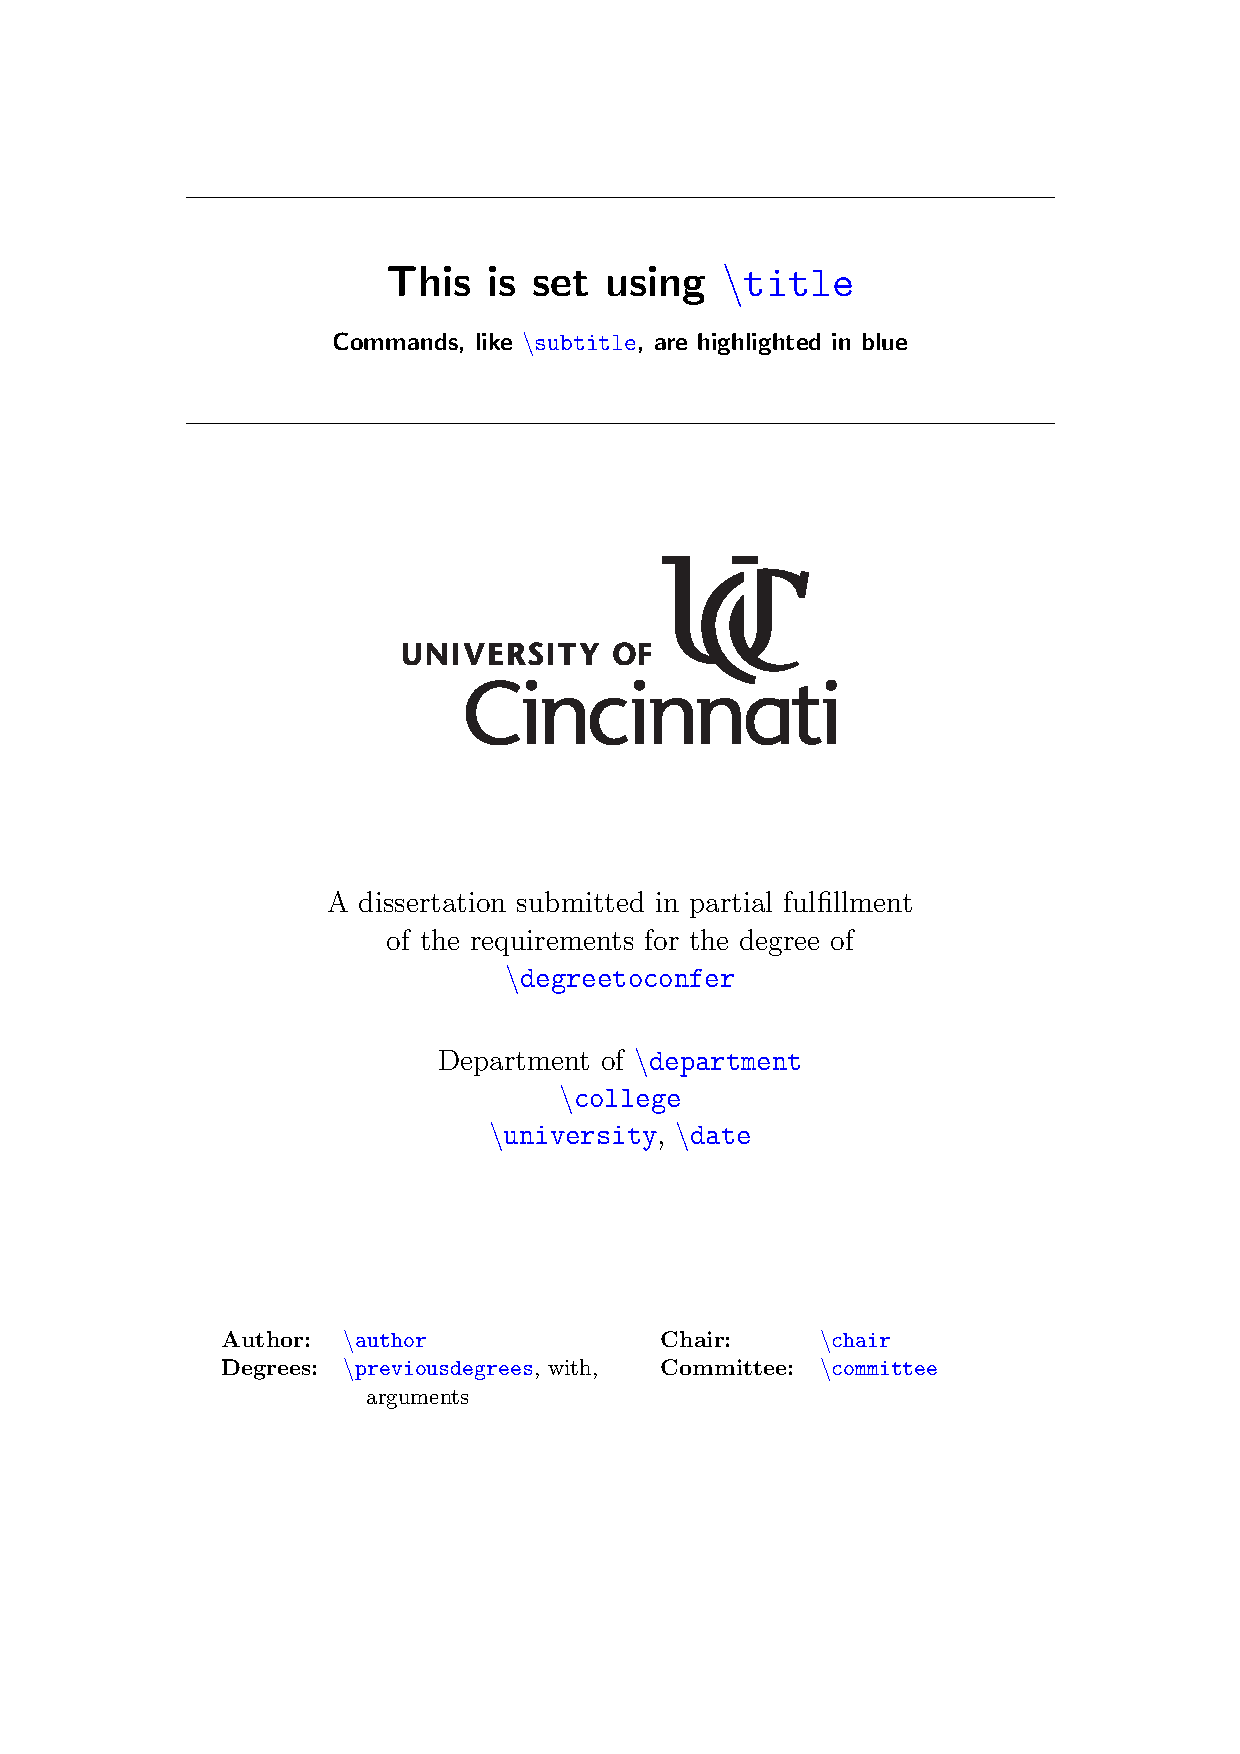
\includegraphics[width=0.7\linewidth]{titlepage-commands.pdf}
  }
  \caption{User input and the title page}
  \label{fig:titlepage}
\end{figure}

The remaining four commands that apply to the title page are set within two tabular environments. 
Therefore, it is important not to place extraneous newline symbols {\color{red}\verb!\\!} or alignment characters {\color{red}\verb!&!} in their arguments.

The author command also takes a single mandatory argument, but this should consist only of alphabetic characters, accents, whitespace,  and possibly punctuation. 
No line break characters should be present since it will be placed in a \verb!tabular! environment with multiple columns.
\begin{lstlisting}
\author{|<author-name>|}
\end{lstlisting}
Punctuation is acceptable if needed. 
For example, \lstinline!\author{Henry Jones, Jr.}! is a valid use of the command. 
However, while usage that includes titles, such as \lstinline!\author{Henry Jones, Jr., Ph.D.}!, will not produce errors, such usage is not recommended because a list of the degrees earned will also appear on the title page. 
On the other hand, if you are a knight in the Order of the British Empire, you may place `KBE' at the end of your name in order to sound pretentious. 

In order to include a list of the previous degrees earned on the title page, the command \lstinline!\previousdegrees! is included, which takes one optional and three mandatory arguments. 
\begin{lstlisting}
\previousdegrees[+<#degrees>+]{|<degrees>|}{|<years>|}{|<schools>|}
\end{lstlisting}
In the above, \lstinline!|<degrees>|!, \lstinline!|<years>|!, and \lstinline!|<schools>|! are semicolon separated lists, and \lstinline!+<#degrees>+! is the number of previous degrees earned (default: 1). 
The information stored is carefully formatted to be placed inside a \verb!tabular! environment and so should not contain an extraneous characters.
I suspect that \lstinline!\previousdegrees! will be the first command to cause serious problems with the layout of the title page for various people since it is the command which manipulates the most information and tries to typeset it in a rather small area.

The \lstinline!\chair! command takes as its sole mandatory argument the name (and title) of your dissertation committee chair. 
\begin{lstlisting}
\chair{|<advisor>|}
\end{lstlisting}
This person should be your advisor. 
Note that unlike in the \lstinline!\degreetoconfer! command, it is important to abbreviate titles. 
For example, correct usage of this command could be: \lstinline!\chair{Random Advisor, PhD}!. 
Unlike the way I have been abbreviating degree names elsewhere in this documentation, the University of Cincinnati style guidelines stipulate that such abbreviations should \emph{not} include periods. 
If your advisor holds multiple degrees, consult them on the appropriate way to reference them on the title page (but undergraduate degrees are not relevant here). 

The last command, \lstinline!\committee! takes one optional and one mandatory argument. 
Its purpose is to list the members of your dissertation committee \emph{other than the committee chair}.
\begin{lstlisting}
\committee[+<#members>+]{|<members>|}
\end{lstlisting}
The optional argument \lstinline!+<#members>+! is simply the number of members on the committee, while the mandatory argument \lstinline!|<members>|! is a semicolon separated list of their names (and titles). 
An example of appropriate usage of this command is
\begin{lstlisting}
\committee[2]{First Member, PhD; Second Member, PhD}
\end{lstlisting}
Note that there is no problem with the space prior to \verb!Second! in the above example; such spaces should be trimmed prior to insertion in the title page. 

Finally, for students outside of the University of Cincinnati who wish to use this class, you may want to use another logo.
This can be achieved through the \lstinline!\logo! command. 
This takes one optional and one mandatory argument, both of which are passed directly to the \lstinline!\includegraphics! command. 
Obviously, the inclusion of the logo at all, whether UC or otherwise, requires \verb!graphicx! package.
Since \verb!graphicx! does not declare any file formats in the class file, you must either do this yourself or use an encapsulated post-script (\verb!eps!) image.
A note to UC students: please don't change the size of the logo using the \lstinline!\logo! command; UC has very strict \href{http://www.uc.edu/content/dam/uc/ucomm/docs/UCBrandingStandards.pdf}{branding standards} regarding usage of the logo. 
The current size, relative position, and spacing of the logo meet these standards, but increasing or decreasing the size, aspect ratio, or position may violate them.

\section{Authoring a dissertation with \LaTeX}

\subsection{Separation of form and content}

Finally, we should make some sort of note about writing long documents (including dissertations and books with \LaTeX. 
One of the tremendous features of \LaTeX{} is the ability to separate \emph{form} from \emph{content}. 
This takes place on two levels: the class definition and the authored files. 
The class defines things like the format of titles, section headings, header and footer material, \textit{et cetera}. 
Then, when the author issues commands like \lstinline!\maketitle! or \lstinline!\section!, he need not worry about how it will \emph{look}, only what he must \emph{say}. 
Of course, if the author has any quibbles with the nuts and bolts of the formatting the class file implements, he may always modify these items to his liking. 
He does this, however, on a project-wide scale instead of locally, at each occurrence of a section heading.

For many projects, such as research articles submitted to peer-reviewed journals, this mild separation of form from content is generally sufficient, and the author may content himself to create a single \verb!tex! file perhaps along with a \verb!bib! Bib\TeX{} file for the references. 

For large projects, however, it is desirable to have more modularity. 
In particular, it is helpful for the author to create a single \emph{master} file which takes care of the general formatting such as: where to place the table of contents, what constitutes front matter, main matter and back matter, where to place the bibliography, glossary, index, \emph{et cetera}, and the design of each. 
This master project file then has many \emph{children}, each of which consists somehow of the main content of the document.
These children are then inserted into the master using either the \lstinline!\input! or \lstinline!\include! commands. 
For a good discussion of the differences between these two commands see this \TeX.SX  \href{http://tex.stackexchange.com/questions/246/when-should-i-use-input-vs-include}{question}. 

The template dissertation included with the \verb!uc-dissertation! document class aims to be as modular as is reasonably helpful. 
Chapters have their own \verb!tex! files and are inserted into the master file \verb!dissertation.tex! via \lstinline!\include!. 
Other items, such as the glossary definitions, also have their own file which is inserted via \lstinline!\input!. 
We highlight this further in what follows. 
For more information on the modular abilities afforded by \LaTeX{}, please see the \href{http://en.wikibooks.org/wiki/LaTeX/Modular_Documents}{\LaTeX{} Wikibook}.

\subsection{The \texttt{uc-disseration} template}

We describe the (simplified) contents of the master file \verb!dissertation.tex! below. 
The preamble is short, calling only the necessary packages and using the few commands necessary. 

The \verb!makeidx! and \verb!glossaries! packages are necessary for, you guessed it, the index and the glossary (the glossaries package is also what we use to create the Notation, or List of Symbols, page via the \lstinline!\newglossary! command). 
The \lstinline!\makeindex! and \lstinline!\makeglossaries! commands are used to create the auxiliary files \LaTeX{} uses. 
These must be built with the \verb!makeindex! (or \verb!xindy! or \verb!texindy!) and \verb!makeglossaries! engines. 
Note how we use modularity to our advantage by putting the definitions of the glossary terms in their own file and then just insert this file into the document with the command
\begin{lstlisting}
%%% Glossary entries
\newglossaryentry{dissertation}{%
  name={dissertation}, 
  description={the culmination of several years of work produced by a lowly Ph.D.~candidate}
}
\newglossaryentry{literature}{%
  name={literature}, 
  description={the body of published knowledge in a given field of study}
}

%%% Symbol List entries
\newglossaryentry{sym-natural}{name={$\mathbb{N}$}, description={the positive integers, also known as the \emph{natural numbers} to mathematicians and computer scientists}, type=symbol}


%%% Local Variables: 
%%% mode: latex
%%% TeX-master: "dissertation"
%%% End: 

\end{lstlisting}
If you have no need of these items in your dissertation, you are welcome to get rid of them and the commands used later to insert them into the document (\lstinline!\printglossary! and \lstinline!\printindex!).

The \verb!biblatex! package is used to typeset the bibliography. 
Note that this package isn't strictly \emph{necessary}, but it is often preferred (over simple Bib\TeX{}) for its ease of customization. 
If you decide to use Bib\TeX{}, you should run the \verb!bibtex8! engine on your document, and if you use Bib\LaTeX{} then it is recommended that you use \verb!biber!.
The main downside of Bib\LaTeX{} as opposed to Bib\TeX{} is a lack of support from publishers. 
This is only a downside for documents you plan to submit to a publisher, but your dissertation is probably not among such documents. 
For more discussion about the difficulties of submitting an article using Bib\LaTeX{} to a journal, please consult this \href{http://tex.stackexchange.com/questions/12175/biblatex-submitting-to-a-journal/12179#12179}{answer} and the resulting comments on \TeX{}.SX. 

\begin{lstlisting}[frame=single,title={The \texttt{dissertation.tex} preamble}]
\documentclass[chap,comply,bibliography=totoc]{uc-dissertation}

\usepackage[style=alphabetic,firstinits=true,maxnames=10]
  {biblatex}
% For glossary, index and list of symbols
\usepackage{makeidx}
\usepackage[toc]{glossaries}
% For reformatting the ToC, LoF, LoT
\usepackage{tocstyle}
\usetocstyle{standard}

%%%%% Set bibliography file(s)
\addbibresource{references.bib}

%%%%% Add symbol list
\newglossary[sbg]{symbol}{sbi}{sbo}{Notation}

%%%%% Make glossary, index and symbol list
\makeindex
\makeglossaries

%%%%% Add the glossary definition file
%%% Glossary entries
\newglossaryentry{dissertation}{%
  name={dissertation}, 
  description={the culmination of several years of work produced by a lowly Ph.D.~candidate}
}
\newglossaryentry{literature}{%
  name={literature}, 
  description={the body of published knowledge in a given field of study}
}

%%% Symbol List entries
\newglossaryentry{sym-natural}{name={$\mathbb{N}$}, description={the positive integers, also known as the \emph{natural numbers} to mathematicians and computer scientists}, type=symbol}


%%% Local Variables: 
%%% mode: latex
%%% TeX-master: "dissertation"
%%% End: 

\end{lstlisting}

\begin{lstlisting}[frame=single,title={\texttt{dissertation.tex} main body}]
\begin{document} 

\frontmatter
%%%%% Set titlepage information

%%% All desired titlepage info must be set before maketitle is called.

\title{This is a title that \\ has multiple lines} 
\subtitle{This subtitle is fairly short}

%% The next command is a redefined date command that takes two
%% arguments of the form {month}{year}, where 'month' is the 
%% two-digit month, and 'year' is the four-digit year. In order 
%% to activate this on the title page you must pass the option 
%% 'fixed' to \maketitle, otherwise it will use \today
\date{05}{2015}
\author{Lowly Candidate}
%% The next command takes 3 mandatory and 1 optional argument.
%% The optional argument is the number of previous degrees held
%% by the candidate and defaults to 1. The mandatory arguments
%% are semicolon separated lists of, respectively, the degrees 
%% held, years obtained, and schools conferring those degrees.
\previousdegrees[3]{%
  B.A. Chemistry; M.S. Physics; M.S. Mathematics }{%
  2000; 2002; 2007 }{%
  University of Somewhere; University of Nowhere; University of Nebraska %
}

\chair{Random Advisor}
%% The next command takes 1 mandatory and 1 optional argument.
%% The optional argument is the number of committee members.
%% defaults to 1. The mandatory argument is a semicolon 
%% separated list of names of the committee members.
\committee[3]{Other Member; Another Member; Y.A. Member}


%% The following commands default to 'Mathematical Sciences',
%% 'McMicken College of Arts and Sciences', and 'University 
%% of Cincinnati' if they are not explicitly set by the user.
\department{Mathematical Sciences}
\college{Eponymous College of Arts and Sciences}
\university{University of Somewhere}

%%% Local Variables: 
%%% mode: latex
%%% TeX-master: "dissertation"
%%% End: 

\maketitle
\abstract{%
This is the abstract.
}

%%% Local Variables: 
%%% mode: latex
%%% TeX-master: "dissertation"
%%% End: 

\abstractpage
\copyrightpage
\acknowledgments{%
This is where we thank people and recognize funding sources.
}
\acknowledgmentspage
\tableofcontents 
\listoftables
\listoffigures
\printglossary[type=symbol]

\mainmatter 
\chapter{Introduction}
\label{cha:introduction}
\chapterquote{Chapter quotes can bring an air of sophistication to your work. Just be sure they aren't signed `anonymous'.}{Anonymous}

\section{Gentle beginnings}

\subsection{The art of introduction}

This is where you give the first \index{impression} impression of your work. 
It is important that it comes across as interesting and worthy of study. 
Make sure you state the major problems you will solve later.
Note that now the material is double-spaced instead of single-spaced (assuming you are using the \verb+comply+ class option).
We will insert a short table so that one appears in the List of Tables.

\begin{table}[h]
  \centering
  \begin{tabular}{c|c}
    $x$ & $y$ \\
    This & That \\
    These & Those \\
    Here & There \\
  \end{tabular}
  \caption{A table to supercede all other tables}
  \label{tab:supercession}
\end{table}

\newpage

\subsection{Harsh second dates}

Unfortunately, not all is well-and-good in the land of make believe dissertations.



%%% Local Variables: 
%%% mode: latex
%%% TeX-master: "dissertation"
%%% End: 

\chapter{Background}

In this chapter we review the literature relevant to our work. 
Here you most likely should have some references \cite{Tol-JoBN-1957}. 

%%% Local Variables: 
%%% mode: latex
%%% TeX-master: "dissertation"
%%% End: 

\chapter{Results}

\chapterquote{God created the integers, all else is the work of man.}{Leopold Kronecker}

This is the \index{chapter} chapter where we prove our main results. This will probably take more than one chapter. Suppose that God created the \index{positive} positive integers \gls{sym-natural} and nothing else, then we can conclude...

%%% Local Variables: 
%%% mode: latex
%%% TeX-master: "dissertation"
%%% End: 


\backmatter
\printglossary
\printbibliography

\mainmattertwo
\appendix
\chapter{Prerequisite material}

We need a figure somewhere, so let's put it here.

\begin{figure}[h]
  \centering
  I'm a float floating away. Float$\ldots$ float$\ldots$ float$\ldots$
  \caption{Hi, I'm a floating figure!}
  \label{fig:floating-stuff}
\end{figure}

%%% Local Variables: 
%%% mode: latex
%%% TeX-master: "dissertation"
%%% End: 


\backmatter
\cleardoublepage
\addcontentsline{toc}{chapter}{Index}
\printindex

\end{document}
\end{lstlisting}

After the preamble, we have the main body of the document. 
Notice how short is this master file. 
That is because all the content has been stripped out and placed in other files, and then is simply inserted via \lstinline!\input! or \lstinline!\include!.

The primary chapters are \verb!introduction!, \verb!background!, \verb!results! and the appendix \verb!prerequisite-material!. 
These are inserted into the document via the \lstinline!\include! command because using this has the option of also calling \lstinline!\includeonly!, which saves time when compiling the document if you are only working on a certain part of the document.
The \lstinline!\include!'d files also have their own \verb!aux! files, which shouldn't be necessary for things like the title page, abstract or acknowledgments pages.


\section{Suggestions}

The KOMA-Script book class \verb!scrbook.cls! (and hence also \verb!uc-dissertation.cls!) typesets section headings in a bold sans serif typeface.
The author may wish to have a coherent style throughout their dissertation and thus would desire to typeset the titles/headings to theorem-like environments in the same way.
This can be achieved by means of the \verb!thmtools! package.
Among many other things, this package allows for the definition and customization of various theorem environment styles.
Below we create an example style which forces the title of the theorem, as well as any accompanying note, to be typeset boldface and san serif.
The other parameters are just included to make it look nice overall.
See the documentation of the \verb!thmtools! package for more details.

\begin{lstlisting}[frame=single,title={\texttt{thmtools} theorem style definition: sans serif}]
\declaretheoremstyle[
  spaceabove=6pt, 
  spacebelow=6pt,
  headfont=\sffamily\bfseries,
  notefont=\sffamily\bfseries, 
  notebraces={(}{)},
  bodyfont=\itshape,
  postheadspace=1em
]{theorem}
\end{lstlisting}

\end{document}


